\documentclass[13pt,oneside]{book}
\usepackage[utf8]{inputenc}
\usepackage{url}
\usepackage{listings}
\usepackage{graphicx}

\usepackage{geometry}
\geometry{a4paper, left=20mm, right=20mm, top=20mm, bottom=20mm}
\usepackage[margin=1.2in]{geometry}
\usepackage[toc,page]{appendix}
\usepackage{graphicx}
\usepackage{natbib}
\usepackage{lipsum}
\usepackage{caption}

\begin{document}

\captionsetup[figure]{margin=1.5cm,font=small,labelfont={bf},name={Figure},labelsep=colon,textfont={it}}
\captionsetup[table]{margin=1.5cm,font=small,labelfont={bf},name={Table},labelsep=colon,textfont={it}}
\setlipsumdefault{1}

\begin{titlepage}
\begin{center}
{\LARGE College Of Engineering Trivandrum}\\[3cm]
\linespread{1.2}\huge {\bfseries System Software Lab}\\[3cm]
\linespread{1}

\includegraphics[width=5cm]{img/emblem.jpeg}\\[3cm]
{\Large GOKUL K\\ S5  CSE \\ Roll No:21\\ TVE18CS021 }\\[1cm]


\textit{ }\\[2cm]
Department of Computer Science\\[0.2cm]
\today
\end{center}

\end{titlepage}

\newpage

\begin{frame}{}
    \centering
    \hspace*{-0.5cm}
    $\vcenter{\hbox{
\includegraphics[width=1.5cm]{img/emblem.jpeg}}}$
    $\vcenter{\resizebox{0.95\textwidth}{!}{
        \begin{tabular}{c}
             CS331 - System Software Lab $\cdot$ 2020 $\cdot$   \\
             \hline 
        \end{tabular}
    }}$
\end{frame}
\section*{Cycle 1}
\section*{Expt 5}
\begin{center}
    \Large{Dining Philosophers Problem}
\end{center}
\section*{Aim}
\large
To implement a program to simulate the working of the dining
philosopher’s problem.

\section*{Algorithm} 
    \begin{verbatim}
		1 process P [ i ]
		2 while true do
		3 { THINK ;
		4 PICKUP ( CHOPSTICK [ i ] , CHOPSTICK [ i +1 mod 5]) ;
		5 EAT ;
		6 PUTDOWN ( CHOPSTICK [ i ] , CHOPSTICK [ i +1 mod 5])
	\end{verbatim}

\section*{Source Code}
\small

\begin{lstlisting}[language=C]
/* Write a program to simulate the working of the dining
philosopher’s problem */

#include <stdio.h>
#include <semaphore.h>
#include <pthread.h>
#include <unistd.h>

#define N 5

typedef enum {
	THINKING,
	HUNGRY,
	EATING
} Actions;

#define LEFT (phil_num + 4) % N
#define RIGHT (phil_num + 1) % N

sem_t mutex;
sem_t S[N];

Actions state[N];
int philosophers[N] = {0, 1, 2, 3, 4}; 

void * philosopher(void *);
void start_eating(int);
void end_eating(int);
void test(int);

void * philosopher(void * num)
{
	while(1)
	{
		int * i = num;
		sleep(1);
		start_eating(*i);
		sleep(0);
		end_eating(*i);
	}
}

void start_eating(int phil_num)
{
	sem_wait(&mutex);
	state[phil_num] = HUNGRY;
	printf("\nPhilosopher%d is hungry", phil_num+1);
	test(phil_num);
	sem_post(&mutex);
	sem_wait(&S[phil_num]);
	sleep(1);
}

void end_eating(int phil_num)
{
	sem_wait(&mutex);
	state[phil_num] = THINKING;
	printf(
		"\nPhilosopher%d stops eating and puts fork %d and %d down",
		phil_num+1,
		LEFT+1,
		phil_num+1
	);
	printf("\nPhilosopher%d is thinking", phil_num+1);
	test(LEFT);
	test(RIGHT);
	sem_post(&mutex);
}

void test(int phil_num)
{
	if(state[phil_num] == HUNGRY && state[LEFT] != EATING && state[RIGHT] != EATING)
	{
		state[phil_num] = EATING;
		sleep(2);
		printf(
			"\nPhilosopher%d takes fork %d and %d",
			phil_num+1,
			LEFT+1,
			phil_num+1
		);
		printf("\nPhilosopher%d is eating", phil_num+1);
		test(LEFT);
		test(RIGHT);
		sem_post(&S[phil_num]);
	}
}

int main()
{
	int i;
	pthread_t thread_id[N];
	sem_init(&mutex, 0, 1);

	for(i = 0; i < N; i++) sem_init(&S[i], 0, 0);

	for(i = 0; i < N; i++)
	{
		pthread_create(&thread_id[i], NULL, philosopher, &philosophers[i]);
		printf("\nPhilosopher%d is thinking", i+1);
	}

	for(i = 0; i < N; i++) pthread_join(thread_id[i], NULL);
}
    \end{lstlisting}
    \section*{Output}
    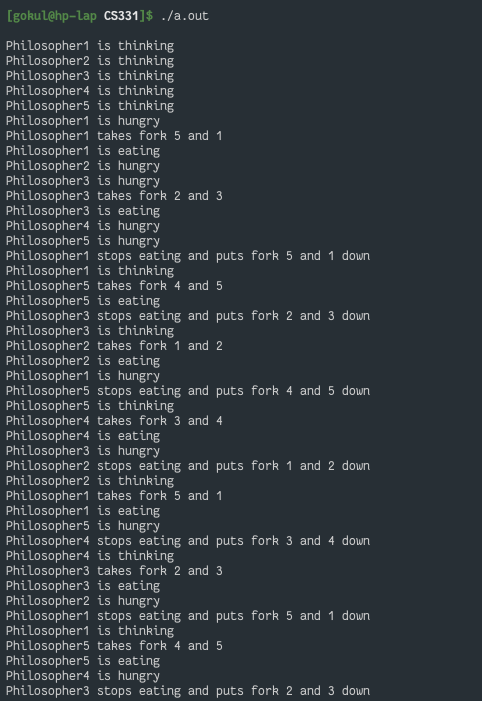
\includegraphics[]{img/p6.png}
    
\Large
\section*{Result}
\large
The dining philosophers problem was solved using semaphores and its output is verified
\end{document}